\documentclass{article}

% ============================================================
% MA 213 In-Class Worksheet Template
% Student-facing worksheet for lecture activities.
% ============================================================

\usepackage[margin=1in]{geometry}
\usepackage{amsmath}
\usepackage{xcolor}
\usepackage{parskip}
\usepackage{array}
\usepackage{enumitem}
\usepackage{booktabs}
\usepackage{graphicx}

\newcommand{\coursenumber}{MA 213}
\newcommand{\weekplaceholder}{11}
\newcommand{\lectureplaceholder}{28}
\newcommand{\lecturetitle}{Beauty and Sex Ratios: Think/Pair/Share}

\newcommand{\nameblank}{\rule{1.75in}{0.4pt}}
\newcommand{\idblank}{\rule{1.55in}{0.4pt}}
\newcommand{\shortblank}{\rule{1in}{0.4pt}}
\newcommand{\longblank}{\rule{0.93\linewidth}{0.4pt}}

\begin{document}

\begin{center}
  {\LARGE \coursenumber{} Week \weekplaceholder{}: Lecture \lectureplaceholder{}}\\
  {\large \lecturetitle{}}
\end{center}

\begin{enumerate}[label=\arabic*.,leftmargin=*,itemsep=.7em]
  \item \textbf{Your name:} \nameblank \hfill \textbf{BU ID:} \idblank
\end{enumerate}

\textbf{Big idea:} A study of $N=2972$ people claimed that the most attractive respondents were 8\% more likely to have a girl than everyone else, and rejected $H_0: d = 0$ at $\alpha = 0.05$. But realistic effect sizes for sex ratios are only about 1\%. The figure below shows the null distribution of the test statistic $\hat{d}$ (centered at 0) alongside the distribution you'd expect if the \emph{true} effect were a more realistic 1\% (centered at 1), both with standard error $\hat\sigma_{\hat d} = 3.3\%$. The dashed lines mark the rejection region boundaries ($\pm 6.5\%$) for a two-sided test at $\alpha = 0.05$.

\begin{center}
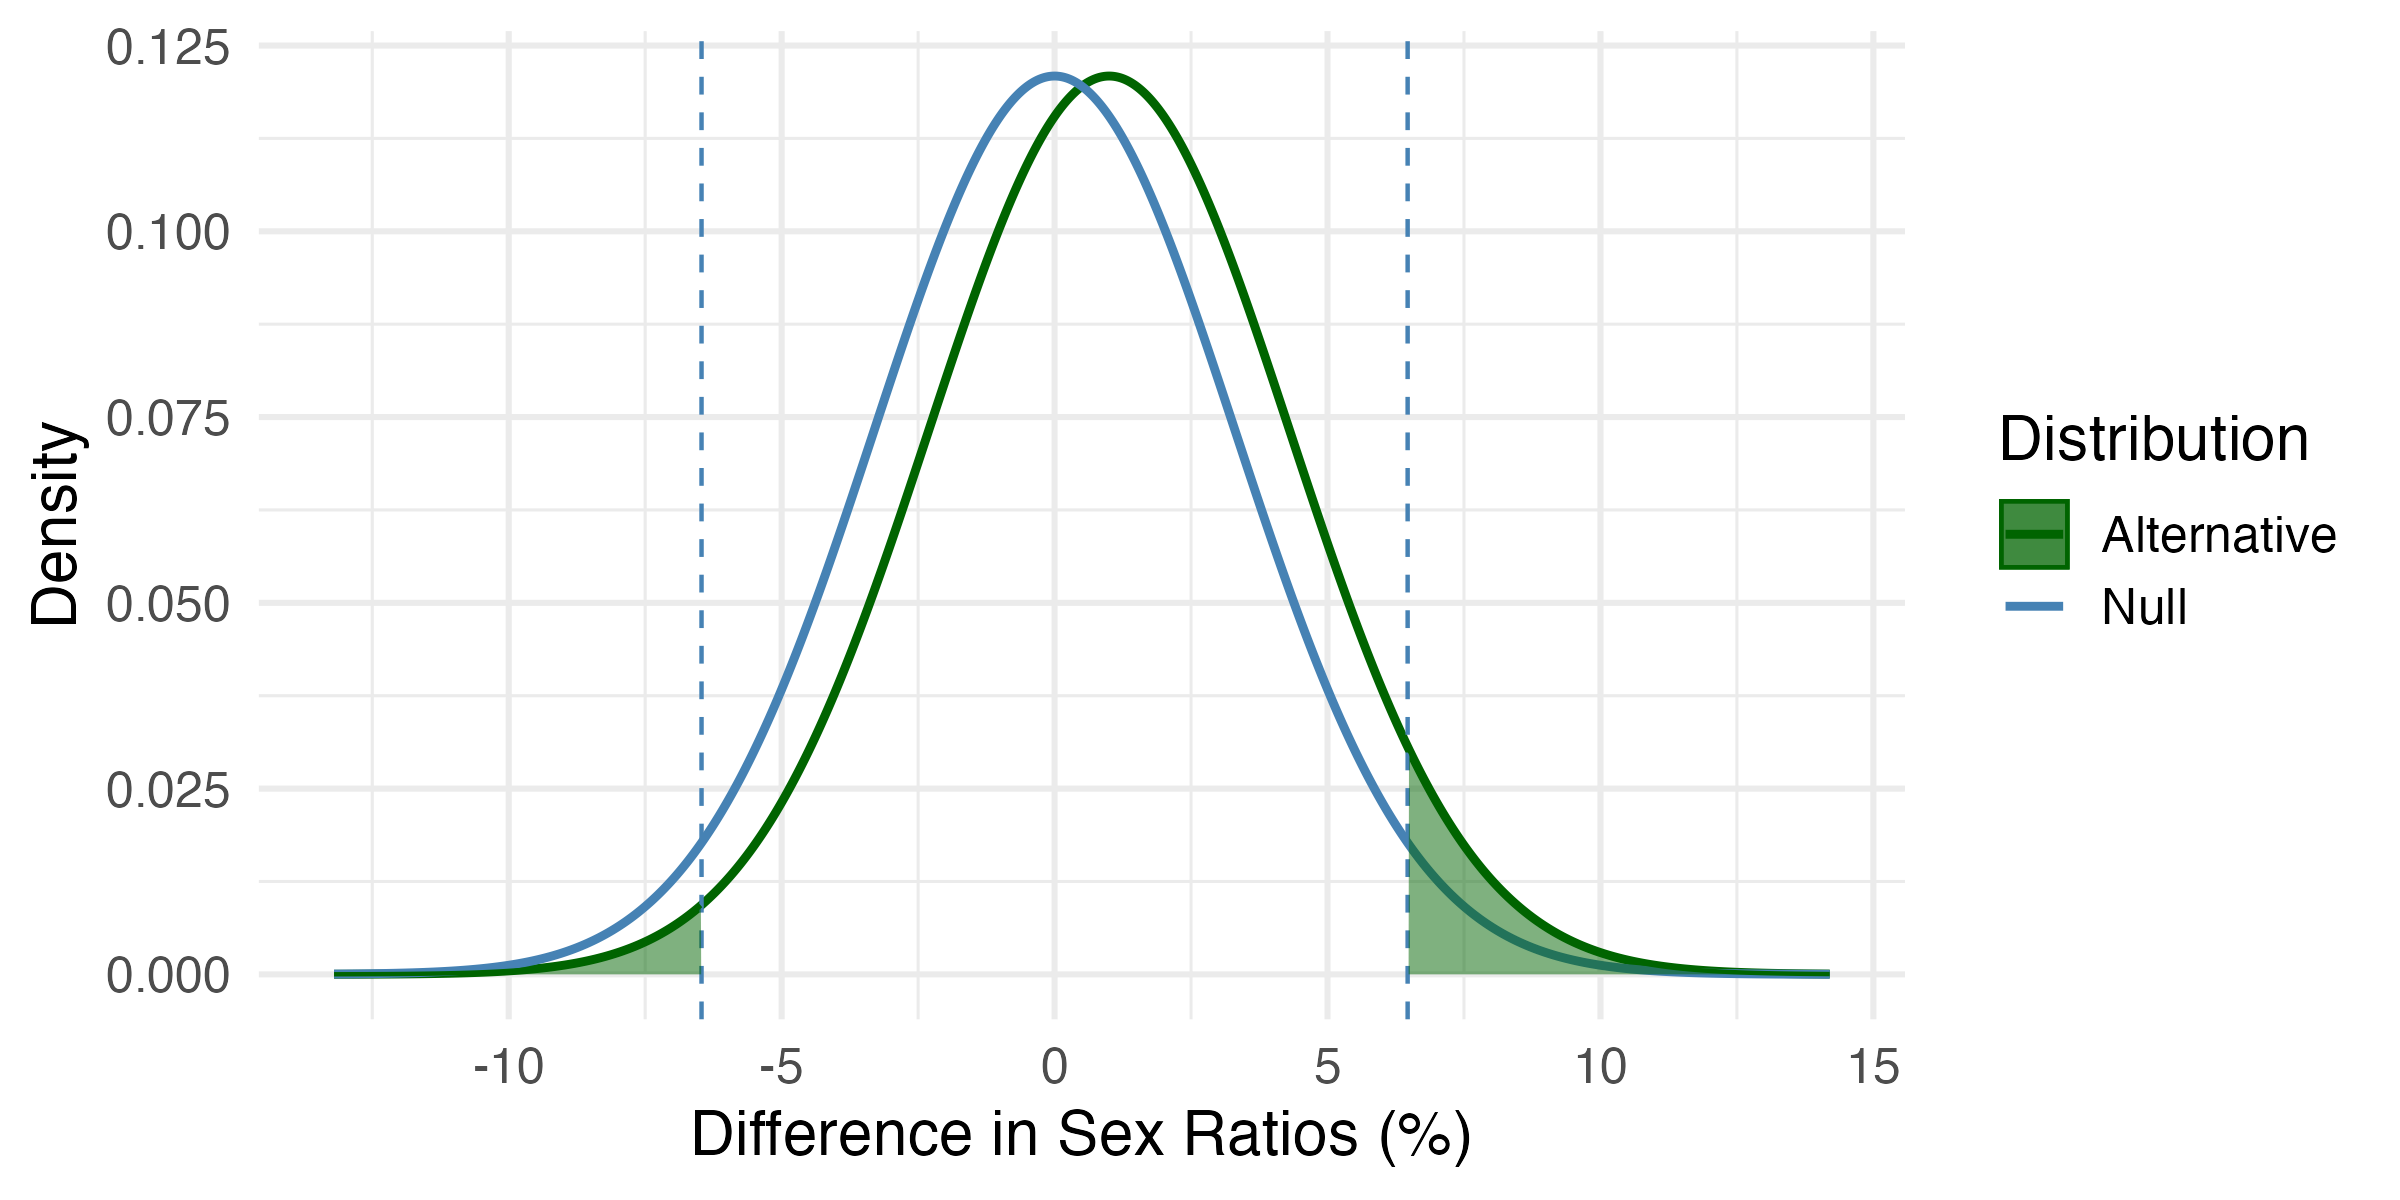
\includegraphics[width=0.75\textwidth]{figures/whatif_sexratio.png}
\end{center}

\section*{Step 1: Think (2 mins)}
Hint: none of these questions require any calculations --- just read the figure and think about what it means.
There are more hints on the next page if you get stuck.

\textbf{(a)} Approximately how big did the difference in sex ratios have to be to reach statistical significance in this study?
\vspace{0.6in}

\textbf{(b)} Approximately what was the power of the test to detect a (realistic) effect of 1\%? (Hint: power is the probability of rejecting $H_0$ when the true effect is 1\%, i.e.\ the area under the \emph{alternative} curve that falls in the rejection region.)
\vspace{0.6in}

\textbf{(c)} If you reject the null hypothesis, what is the approximate probability that your observed difference in sex ratios is in the wrong direction (a sign error)? (Hint: compare the two shaded tails of the alternative curve.)
\vspace{0.6in}

\newpage
\section*{Hints for Step 1}

\textbf{(a)} The dashed lines mark the null (blue) curve's rejection region. 

\vspace{0.2in}

\textbf{(b)} Power is the chance of rejecting $H_0$ \emph{given that the alternative is true}, so it lives entirely on the alternative (green) curve. Visually compare the shaded area under the green curve (both tails, outside the dashed lines) to the green curve's total area. Roughly what fraction is shaded? A rough visual estimate (e.g.\ ``less than 10\%'') is enough --- you don't need an exact number.

\vspace{0.2in}

\textbf{(c)} A sign error means you reject $H_0$, but your observed difference lands in the \emph{left} shaded tail (favoring the wrong direction) rather than the right one. Compare the sizes of the two shaded tails under the green curve: the sign-error probability is roughly (left tail) $\div$ (left tail $+$ right tail), i.e.\ what share of \emph{all} significant results would land on the wrong side.

\vspace{0.2in}
\noindent\rule{\linewidth}{0.4pt}
% \vspace{0.2in}

\section*{Step 2: Pair (2 mins)}

\begin{enumerate}[label=\arabic*.,leftmargin=*,itemsep=.7em, start=2]
  \item \textbf{Partner's name:} \nameblank \hfill \textbf{BU ID:} \idblank
\end{enumerate}

Compare your estimates with your partner. Then discuss:

\begin{itemize}
  \item Given how low the power is, what does it mean that this study \emph{did} reject $H_0$? Should you trust the reported 8\% effect?
  \item What would you tell the researchers to do differently in a follow-up study?
\end{itemize}

\textbf{Our thoughts:}
\vfill

\end{document}
